\documentclass[]{article}
\usepackage{mathptmx}
\usepackage{booktabs}
\usepackage{tabularx}
\usepackage{graphicx}
\usepackage{circuitikz}
\usepackage{tikz-timing}
\usepackage{todonotes} 
\usepackage{setspace}
\newcounter{mycmtctr}
\newcommand{\mycomment}[2][]
{
    % initials of the author (optional) + note in the margin
    \refstepcounter{mycmtctr}%
    {%
        \setstretch{0.7}% spacing
        \todo[color={red!100!green!33},size=\footnotesize]
        {
            \textbf{Comment [\uppercase{#1}\themycmtctr]:}~#2
        }
    }
}
\newcommand{\myinlinecomment}[2][]
{
    % initials of the author (optional) + note inlin
    \refstepcounter{mycmtctr}%
    {%
        \setstretch{0.7}% spacing
        \todo[inline,color={red!100!green!33},size=\footnotesize]
        {
            \textbf{Comment [\uppercase{#1}\themycmtctr]:}~#2
        }
    }
}
\newcolumntype{C}{>{\centering\arraybackslash\hsize=.32\hsize}X}%
\usepackage[T1]{fontenc}
\usepackage{lmodern}
\usepackage{amssymb,amsmath}
\usepackage{ifxetex,ifluatex}
\usepackage{fixltx2e} % provides \textsubscript
% use upquote if available, for straight quotes in verbatim environments
\IfFileExists{upquote.sty}{\usepackage{upquote}}{}
\ifnum 0\ifxetex 1\fi\ifluatex 1\fi=0 % if pdftex
  \usepackage[utf8]{inputenc}
\else % if luatex or xelatex
  \usepackage{fontspec}
  \ifxetex
    \usepackage{xltxtra,xunicode}
  \fi
  \defaultfontfeatures{Mapping=tex-text,Scale=MatchLowercase}
  \newcommand{\euro}{€}
\fi
% use microtype if available
\IfFileExists{microtype.sty}{\usepackage{microtype}}{}
\usepackage{color}
\usepackage{fancyvrb}
\newcommand{\VerbBar}{|}
\DefineShortVerb[commandchars=\\\{\}]{\|}
\DefineVerbatimEnvironment{Highlighting}{Verbatim}{commandchars=\\\{\}}
% Add ',fontsize=\small' for more characters per line
\usepackage{framed}
\definecolor{shadecolor}{RGB}{248,248,248}
\newenvironment{Shaded}{\begin{snugshade}}{\end{snugshade}}
\newcommand{\KeywordTok}[1]{\textcolor[rgb]{0.13,0.29,0.53}{\textbf{{#1}}}}
\newcommand{\DataTypeTok}[1]{\textcolor[rgb]{0.13,0.29,0.53}{{#1}}}
\newcommand{\DecValTok}[1]{\textcolor[rgb]{0.00,0.00,0.81}{{#1}}}
\newcommand{\BaseNTok}[1]{\textcolor[rgb]{0.00,0.00,0.81}{{#1}}}
\newcommand{\FloatTok}[1]{\textcolor[rgb]{0.00,0.00,0.81}{{#1}}}
\newcommand{\CharTok}[1]{\textcolor[rgb]{0.31,0.60,0.02}{{#1}}}
\newcommand{\StringTok}[1]{\textcolor[rgb]{0.31,0.60,0.02}{{#1}}}
\newcommand{\CommentTok}[1]{\textcolor[rgb]{0.56,0.35,0.01}{\textit{{#1}}}}
\newcommand{\OtherTok}[1]{\textcolor[rgb]{0.56,0.35,0.01}{{#1}}}
\newcommand{\AlertTok}[1]{\textcolor[rgb]{0.94,0.16,0.16}{{#1}}}
\newcommand{\FunctionTok}[1]{\textcolor[rgb]{0.00,0.00,0.00}{{#1}}}
\newcommand{\RegionMarkerTok}[1]{{#1}}
\newcommand{\ErrorTok}[1]{\textbf{{#1}}}
\newcommand{\NormalTok}[1]{{#1}}
\usepackage{graphicx}
% We will generate all images so they have a width \maxwidth. This means
% that they will get their normal width if they fit onto the page, but
% are scaled down if they would overflow the margins.
\makeatletter
\def\maxwidth{\ifdim\Gin@nat@width>\linewidth\linewidth
\else\Gin@nat@width\fi}
\makeatother
\let\Oldincludegraphics\includegraphics
\renewcommand{\includegraphics}[1]{\Oldincludegraphics[width=\maxwidth]{#1}}
\ifxetex
  \usepackage[setpagesize=false, % page size defined by xetex
              unicode=false, % unicode breaks when used with xetex
              xetex]{hyperref}
\else
  \usepackage[unicode=true]{hyperref}
\fi
\hypersetup{breaklinks=true,
            bookmarks=true,
            pdfauthor={Rohit Ramesh},
            pdftitle={Introduction To Embedded Systems Development},
            colorlinks=true,
            urlcolor=blue,
            linkcolor=magenta,
            pdfborder={0 0 0}}
\urlstyle{same}  % don't use monospace font for urls
\setlength{\parindent}{0pt}
\setlength{\parskip}{6pt plus 2pt minus 1pt}
\setlength{\emergencystretch}{3em}  % prevent overfull lines
\setcounter{secnumdepth}{5}


\title{Introduction To Embedded Systems Development}
\author{Rohit Ramesh}
\date{}

\begin{document}
\maketitle

{
\hypersetup{linkcolor=black}
\setcounter{tocdepth}{2}
\tableofcontents
}
\newpage

\section{Introduction}

This class will teach you about the LPC1769, an ARM Cortex
microcontroller. When compared to normal CPU the LPC is a simple device,
with only one processor core and a miniscure amount of memory, it still
manages to be useful. In fact this simplicity makes it a wonderful
learning tool, allowing us to forgo kernel and driver interfaces and
work at the lowest level possible, without coming too complicated to
just dive into. We'll exploit this to teach you about how processors are
structured, how to deal with many common protocols and tools, and even
how some of the most fundamental parts of an operating system work.

The LPC itself has a number of modules, which encapsulate various
features of the processor. We'll be working our way through those
modules, explaining why you would use them, how they work, and how to
use them. With each module we learn about, we'll present execises and
projects that will help you cement that knowledge, and give you a
practical examples of how these devices can be used.

While we'll often be working with electronics, no initial knowledge is
required, and we'll give you the resources to learn what you need to
know as you go along.

\subsection{Resources}

This textbook will mainly work to help you build a conceptual framework
around these topics, there are other resources that will give you the
fine detail.

\subsubsection{The LPC 17XX User Manual}

The User Manual
(\href{http://www.nxp.com/documents/user_manual/UM10360.pdf}{available
here}\footnote{\url{http://www.nxp.com/documents/user_manual/UM10360.pdf}})
will be the main document this textbook builds on. It contains detailed
information on all of the available features of the LPC, and how you can
use them.

Though this textbook is meant to give you all of the background that the
manual lacks, it is in no way a substitute. There will be a lot we
cannot actually go over and to get the most out of this course, after
every chapter you read in this textbook, you should read the
corresponding chapters in the manual.

\subsubsection{The LPC1769 Schematic}

The schematic
(\href{http://www.cs.umd.edu/class/fall2012/cmsc498a/manuals/lpcxpresso_lpc1769_schematic.pdf}{available
here} \footnote{\url{http://www.cs.umd.edu/class/fall2012/cmsc498a/manuals/lpcxpresso_lpc1769_schematic.pdf}})
is the only way to know how the pins on the dev boards we work with
correspond to the pins mentioned in the manual. You'll need to cross
reference this schematic with Chapter 8 of the manual every time you
need to figure out the physical location of any one particular pin.

\subsubsection{The LPC176X Data Sheet}

The data sheet
(\href{http://www.nxp.com/documents/data_sheet/LPC1769_68_67_66_65_64_63.pdf}{available
here}\footnote{\url{http://www.nxp.com/documents/data_sheet/LPC1769_68_67_66_65_64_63.pdf}})
is the last reference document you should keep handy. It contains a lot
of information about the limitations of the LPC, the tolerances of
various features, and the full set of features the LPC has.

\newpage

\section{GPIO}

\subsection{Prequisites}

Read the following tutorials to get you up to speed with the
electronics:

\begin{itemize}
\itemsep1pt\parskip0pt\parsep0pt
\item
  \href{https://learn.sparkfun.com/tutorials/how-to-read-a-schematic}{How
  to read a schematic}
\item
  \href{https://learn.sparkfun.com/tutorials/how-to-use-a-breadboard/introduction}{How
  to use a breadboard}
\item
  \href{https://learn.sparkfun.com/tutorials/light-emitting-diodes-leds}{Understanding
  LEDs}
\item
  \href{https://learn.sparkfun.com/tutorials/pull-up-resistors/introduction}{Using
  Pull Up Resistors}
\end{itemize}

All these tutorials are Arduino centric, but you should be able to
easily extrapolate to what you need to do for your LPC.

\subsection{What is GPIO?}

We'll start with the most basic peripheral on the LPC, General Purpose
Input Output. GPIO is what lets your microcontroller be something more
than a weak auxiliary processor. With it you can interact with the
outside world, connecting up all manner of tools and turning your
microcontroller into something useful.

GPIO has two fundamental operating modes, input and output. Input lets
you read the voltage on a pin, to see whether it's held low (0v) or high
(3v) and deal with that information programmatically. Output lets you
set the voltage on a pin, again either high or low. Every pin on the LPC
can be used as a GPIO pin, and can be independently set to act as an
input or output.

In this chapter we will show how to complete 2 tasks, reading the state
of a button, and making an LED blink. Using what you learn from that,
you'll be able to start building more complex devices, and even
implementing simple communications protocols.

\subsection{GPIO Output}

GPIO output is an incredibly versatile and powerful tool, especially
given that it takes little effort to use and control it. Once you've
chosen a pin, the process to use it is straighforward; first you tell
the LPC that the pin should be used as an output, and then you tell the
LPC whether the pin should be held low or high. The interesting part is
how exactly you can give the LPC instructions, and what it does in order
to carry them out.

\subsubsection{Memory Mapped Registers}

In order to talk to the GPIO controller, or any other peripheral, we
have we have to use \emph{memory mapped registers}. In most computers
these low level interfaces are hidden by the kernel, and often only
higher level interfaces are available to developers. The LPC however
doesn't have a kernel or drivers hiding these interfaces from you. This
gives you the ability to work with them directly, without having to deal
with the extra complexity an OS would add.

When we try to read or write to a normal chunk of memory, the address
and instruction are sent to the memory controller. The memory controller
then either retrieves data from memory and places it into a register, or
takes data from a register and writes it to somewhere in the memory.
However, there are a number of privileged address, and when you try to
read from or write to these a slightly different pathway is taken. Here
when the memory controller gets the instruction it notices the address
is special, and instead of going to the memory module, it'll forward the
request to a register that's located in the relevant peripheral.

These registers all have different functions, each of which is detailed
in the manual along with the register's memory address. The really
important thing to notice is that you're not dealing with a normal piece
of memory, and these memory mapped registers can act very differently.

Unlike static memory where you can read or write pretty much anywhere,
there are a number of these memory mapped registers which you can only
read from. Trying to write to any of these will trap your system in a
hard fault. Neither can you rely on the assumption that reads are
nondestructive. There are some registers which are connected to FIFOs
and other structures, and reading from them is the same as popping from
that queue, and the next time you read from the same address, you'll get
a different value. Even the usual guarantee that a write operation is
idempotent is lost. There are registers where a write operation will
trigger some change in the peripheral, making the LPC turn an LED on, or
send out a signal.

\subsubsection{Blinking Lights}

So let's start with something simple: Blinking Lights. Connect up an LED
to pin \texttt{P0{[}9{]}} and ground, making sure to place the proper
current limiting resistor in series with it. To actually turn on the LED
you have to first tell the LPC that the pin is to be used for output,
and then set the state to be on. If you look in the manual you'll see
that \texttt{P0{[}9{]}}'s direction is controlled by the 9th bit in a
register located at \texttt{0x2009C000}, and that setting it to 1 makes
it an output pin. \todo[size=\footnotesize]{Add cite for manual p.107}

\begin{Shaded}
\begin{Highlighting}[]
    \NormalTok{((}\DataTypeTok{uint32_t} \NormalTok{*) }\BaseNTok{0x2009C000}\NormalTok{) |= (}\DecValTok{1} \NormalTok{<< }\DecValTok{9}\NormalTok{); }\CommentTok{// Set P0[9] to output}
\end{Highlighting}
\end{Shaded}

Then there's another register at \texttt{0x2009C014} which controls the
state of the pin, so we can turn turn the light on and off by
manipulating its 9th bit.

\begin{Shaded}
\begin{Highlighting}[]
    \NormalTok{((}\DataTypeTok{uint32_t} \NormalTok{*) }\BaseNTok{0x2009C014}\NormalTok{) |= (}\DecValTok{1} \NormalTok{<< }\DecValTok{9}\NormalTok{);  }\CommentTok{// Turn On}
    \NormalTok{((}\DataTypeTok{uint32_t} \NormalTok{*) }\BaseNTok{0x2009C014}\NormalTok{) &= ~(}\DecValTok{1} \NormalTok{<< }\DecValTok{9}\NormalTok{); }\CommentTok{// Turn Off}
\end{Highlighting}
\end{Shaded}

So now you should be able to make the light blink, or by varying the
amount of time on and off, let it glow with varying levels of
brightness.

\subsubsection{An Easier Way}

Of course writing out the memory address every time you wish to change a
register isn't easy, or readable. You could replace it with a
preprocessor macro, but writing those macros would be painful and
tedious. Thankfully there's already a library of macros and structures
that already exists, and which exploits the fact that the memory
addresses for each single peripheral are laid out close together, and
are tightly packed.

CMSIS is a library written by engineers at NXP, and it sets up all these
memory addresses as macros for you. To see how it works let's look at
the setup for the DAC (Digital to Analog Converter). The DAC is a device
which can take a digital value, and turns it into an analog output, it's
controlled with only 3 registers, the functions of which we'll look at
in a later chapter. In \texttt{LPC17xx.h} you'll find a long list of
struct definitions and a series of raw memory addresses. The addresses
point to the chunks of memory assigned to each peripheral and the
structs show the layout of each of those chunks of memory.

\begin{Shaded}
\begin{Highlighting}[]
    \CommentTok{/*----- Digital-to-Analog Converter (DAC) ------*/}
    \KeywordTok{typedef} \KeywordTok{struct}
    \NormalTok{\{}
        \NormalTok{__IO }\DataTypeTok{uint32_t} \NormalTok{DACR;}
        \NormalTok{__IO }\DataTypeTok{uint32_t} \NormalTok{DACCTRL;}
        \NormalTok{__IO }\DataTypeTok{uint16_t} \NormalTok{DACCNTVAL;}
    \NormalTok{\} LPC_DAC_TypeDef;}

        \NormalTok{...}

    \OtherTok{#define LPC_APB1_BASE (0x40080000UL)}
        \NormalTok{...}

    \OtherTok{#define LPC_DAC_BASE  (LPC_APB1_BASE + 0x0C000)}

        \NormalTok{...}

    \OtherTok{#define LPC_DAC       ((LPC_DAC_TypeDef *) LPC_DAC_BASE )}
\end{Highlighting}
\end{Shaded}

The DAC is an APB1\footnote{APB stands for Applied Peripheral Bus, there
  are two in the LPC and some peripherals are connected to each.}
peripheral and so \texttt{LPC\_DAC\_BASE} is the start of the memory
mapped to DAC registers. \texttt{LPC\_DAC\_Typedef} is a struct that's
set up so that when it's aligned to that base address, each of the
struct's fields will align with a particular register in the DAC memory
space. This whole setup means that you can write to the DAC Control
Registers without using a raw memory location.

\begin{Shaded}
\begin{Highlighting}[]
    \NormalTok{LPC_DAC->DACCTRL = }\CommentTok{/* stuff */}\NormalTok{;}
\end{Highlighting}
\end{Shaded}

If you look back at the code we wrote for LED manipulation, and refactor
it, you'll get something much easier to work with.

\begin{Shaded}
\begin{Highlighting}[]
    \NormalTok{LPC_GPIO0->FIODIR |= (}\DecValTok{1} \NormalTok{<< }\DecValTok{9}\NormalTok{);  }\CommentTok{// Set P0[9] to write}
    \NormalTok{LPC_GPIO0->FIOPIN |= (}\DecValTok{1} \NormalTok{<< }\DecValTok{9}\NormalTok{);  }\CommentTok{// Turn LED on}
    \NormalTok{LPC_GPIO0->FIOPIN &= ~(}\DecValTok{1} \NormalTok{<< }\DecValTok{9}\NormalTok{); }\CommentTok{// Turn LED off}
\end{Highlighting}
\end{Shaded}

Having a layer of macros like this also makes it easier to port your
code to another platform, since you'll have to only change the macro
definitions rather than all the pieces of code which use some registers.

\subsubsection{More Registers}

If you look closely there's 4 GPIO ports, each controlling up to 32
pins, and each of those blocks has 5 registers. Strictly speaking you
only need the \texttt{FIODIR} (set pin direction) and \texttt{FIOPIN}
(set or read pin state) registers to control each pin, but there are
three others, which allow you to perform operations much faster.

\texttt{FIOSET} and \texttt{FIOCLR} are the two fast output control
registers.\footnote{The fast in their moniker refers to the fact that
  using them takes fewer operations than using \texttt{FIOPIN}.} Writing
a 1 to a bit in \texttt{FIOSET} will enable the corresponding pin, and
writing to \texttt{FIOCLR} will disable the pin.

\begin{Shaded}
\begin{Highlighting}[]
    \NormalTok{LPC_GPIO0->FIOSET = }\DecValTok{1} \NormalTok{<< }\DecValTok{9}\NormalTok{; }\CommentTok{// Turn LED On}
    \NormalTok{LPC_GPIO0->FIOCLR = }\DecValTok{1} \NormalTok{<< }\DecValTok{9}\NormalTok{; }\CommentTok{// Turn LED Off}
\end{Highlighting}
\end{Shaded}

\texttt{FIOSET} is a good example of how the usual guarantees of memory
structure are lost when working with memory mapped data. Writing a 1 to
\texttt{FIOSET} will set the corresponding bit in \texttt{FIOPIN} to 1,
while writing a 0 will do nothing. In effect `\texttt{FIOSET = ...}' is
an alias for `\texttt{FIOPIN \textbar{}= ...}'. However reading from
\texttt{FIOSET} is a completely different action, it will return the
value from the output state register, a register which stores the
current output value for all the pins, regardless of whether they are
current being used as such.

Writes to \texttt{FIOCLR} can be similarly thought of as an alias, in
this case from `\texttt{FIOPIN \&= \textasciitilde{} ...}' to
`\texttt{FIOCLR = ...}'. But reading from \texttt{FIOCLR} is undefined,
there is simply nothing that operation can look at when pointed at
\texttt{FIOCLR}.

This idea of memory mapped registers being aliases for more complex
commands hints at why these registers are called the ``\emph{fast}
output control registers''. Trying to change the value of a single pin
with \texttt{FIOPIN} requires at least 3 operations operations, a read ,
a bitwise logic operation, and a write. To make the same change using
the fast registers requires only a write operation, the rest of the
stuff is done in hardware, which can be much faster.

\texttt{FIOMASK} is, in effect, a filter for
\texttt{FIOPIN},\texttt{FIOSET}, and \texttt{FIOCLR}. If a bit in
\texttt{FIOMASK} is a 1, then none of those registers can cause any
change in that pin's state. This means that you can change a subset of
the bits very quickly, without having to perform a masking operation
every time. By default all of \texttt{FIOMASK}'s bits are set to 0,
meaning that the other control registers can operate freely.

\subsection{GPIO Input}

Reading a pin uses the same registers we've already used, once a pin's
mode is set to input in \texttt{FIODIR}, the corresponding bit in
\texttt{FIOPIN} holds the currently read value. In addition to simply
reading the registers to figure out the voltage on a pin, we've also got
access to interrupts, which will notify your program when the state of a
pin changes, while allowing you to do something else in the meantime.

\subsubsection{Basics}

Reading the current state of a pin in the middle of your code is simple,
we take the same two registers as before \texttt{FIODIR} and
\texttt{FIOPIN}, and use them slightly differently.

\begin{Shaded}
\begin{Highlighting}[]
    \NormalTok{LPC_GPIO0->FIODIR &= ~(}\DecValTok{1} \NormalTok{<< }\DecValTok{9}\NormalTok{);          }\CommentTok{// Set P0[9] to Input}
    \NormalTok{PinState = (LPC_GPIO0->FIOPIN >> }\DecValTok{9}\NormalTok{) & }\DecValTok{1}\NormalTok{; }\CommentTok{// Get P0[9] State}
\end{Highlighting}
\end{Shaded}

Here a zero in a particular position in \texttt{FIODIR} means the pin is
used for input, and the relevant bit in \texttt{FIOPIN} contains its
current state. Writes to \texttt{FIOPIN},\texttt{FIOCLR} or
\texttt{FIOSET} don't affect input pins, and making changes to the value
of an input pin is basically a no-op.

Once you have this set up, you can connect up a switch with a pull down
resistor to the input pin, and be able to read the state of your button
in software.

\subsubsection{Bouncing}

So if you want to toggle an LED whenever you press a button you might do
something like the following.

\begin{Shaded}
\begin{Highlighting}[]
    \DataTypeTok{int} \NormalTok{state, prevstate = }\DecValTok{0}\NormalTok{;}
    \KeywordTok{while}\NormalTok{(}\DecValTok{1}\NormalTok{)\{ }
        \CommentTok{// Get state of P0[9]}
        \NormalTok{state = (LPC_GPIO0->FIOPIN >> }\DecValTok{9}\NormalTok{) & }\DecValTok{1}\NormalTok{;  }
        \CommentTok{// If there's a change from 0 to 1}
        \KeywordTok{if}\NormalTok{(!prevstate && state) \{    }
            \CommentTok{// Toggle P0[8]}
            \NormalTok{LPC_GPIO0->FIOPIN ^= }\DecValTok{1} \NormalTok{<< }\DecValTok{8}\NormalTok{;      }
        \NormalTok{\}}
        \NormalTok{prevstate = state;}
    \NormalTok{\}}
\end{Highlighting}
\end{Shaded}

When you try that, you'll notice some odd behavior, not only will the
LED change when you press the button, but it will occasionally also
change when you release the button. Sometimes it'll miss button presses
completely, and not change the LED's state.

\begin{figure}[htbp]
\centering
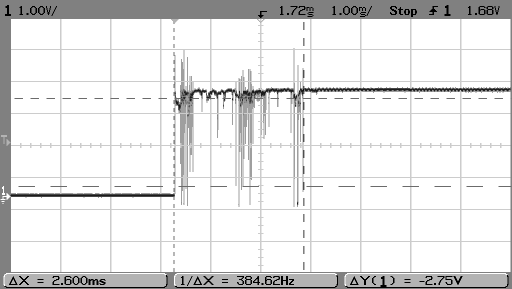
\includegraphics{assets/Bouncy_Switch.png}
\caption{What button presses actually look like.}
\end{figure}

This happens because buttons aren't perfect, and instead of getting
smooth transitions from connected to disconnected, the transitions are
disjointed and shaky, this phenomenon is known as bouncing. Because the
GPIO pins can only read if something is low or high these jitters result
in a number of very fast transitions before the voltage stabilizes. Your
LPC will see some of these transitions as a separate button presses and
toggle the LED accordingly. Most of the time, the bouncing will happen
between reads of the pin state but sometimes, a read will happen in the
middle of the bouncing and cause anomalous output.

Removing the errors caused by bouncing can be done with hardware or
software. In hardware, using a capacitor or a
\href{http://en.wikipedia.org/wiki/Schmitt_trigger}{Schmitt Trigger} can
sometimes solve the problem. In software, one can check if the input has
been stable for a while before acting upon an event. There are also many
other \href{http://www.eng.utah.edu/~cs5780/debouncing.pdf}{ways to deal
with bouncing} that can be more complex but also more reliable.

\subsubsection{Interrupts}

There's another way to get input from GPIO pins, this time without
having to stop and poll the state of your button waiting for something
to happen. With the correct settings the processor can wait for an event
in the background while letting your code run in the meantime. When the
event happens, the processor will interrupt your currently running code,
run code to respond to the event, and restart the execution of your main
program.

These \emph{interrupts} can be very complex and so we're only going to
touch on a small subset of their capabilities. For GPIO specifically, an
interrupt can be triggered when the CPU detects a rising or falling
edge\footnote{A rising edge is the pin's value changing from a 0 to a 1,
  and a falling edge is the value changing from a 1 to a 0.} on an input
pin. Once the edge is detected, the Interrupt Controller performs a
context switch. In this case, saving any of the current registers to the
stack, and starting the executing of the interrupt handler. Once the
interrupt handler is done, the processor will restore the previously
saved registers, and continue executing the original code.

The Interrupt Controller uses an internal flag to determine whether or
not to perform a context switch, and this flag is not automatically
turned off once it has been set. This means that if you don't manually
disable the flag, the interrupt handler will execute repeatedly until
the flag is disabled. \emph{Interrupt chaining} lets you keep your code
small, and modular while still being able to handle many quickly
incoming events. By only disabling the flag for the particular event
you've handled, you are guaranteed to have your interrupt handler called
again, so that it can handle a different event.

\paragraph{Setting Up an Interrupt Handler}

Setting up a GPIO interrupt is another relatively simple process,
starting with telling the NVIC to enable the relevant external
interrupt. Then in the struct \texttt{LPC\_GPIOINT} you'll find the
registers \texttt{IO0IntEnR} and \texttt{IO0IntEnF} which define which
pins on GPIO Port 0 generate interrupts on a rising and falling
edge.\footnote{These registers are for pins on GPIO Port 0. There are
  similar registers with \texttt{IO2} instead for pins on GPIO Port 2.
  The other GPIO ports don't have support for interrupts, and don't have
  interrupt registers.}

\begin{Shaded}
\begin{Highlighting}[]
    \CommentTok{// Turn on External Interrupt 3}
    \NormalTok{NVIC_EnableIRQ(EINT3_IRQn);}
    \CommentTok{// Enable Rising Edge Interrupt on P0[9]}
    \NormalTok{LPC_GPIOINT->IO0IntEnR |= (}\DecValTok{1} \NormalTok{<< }\DecValTok{9}\NormalTok{);}
    \CommentTok{// Enable Falling Edge Interrupt on P0[9]}
    \NormalTok{LPC_GPIOINT->IO0IntEnF |= (}\DecValTok{1} \NormalTok{<< }\DecValTok{9}\NormalTok{);}
\end{Highlighting}
\end{Shaded}

Once the interrupt is enabled and will trigger on the right pins, the
handler has to be defined. The interrupt handlers are found in
\texttt{cr\_startup\_lpc176x.c} in each of your project's source
directories, defined as weak aliases to the default interrupt handler.
Because they're weakly defined, defining a new function with the same
name will make that the handler for the interrupt.

\begin{Shaded}
\begin{Highlighting}[]
    \CommentTok{// Turn on the LED when the button is pressed}
    \DataTypeTok{void} \NormalTok{EINT3_IRQHandler() \{}
        \CommentTok{// If the rising edge interrupt was triggered}
        \KeywordTok{if}\NormalTok{((LPC_GPIOINT->IO0IntStatR >> }\DecValTok{9}\NormalTok{) & }\DecValTok{1}\NormalTok{)\{}
            \CommentTok{// Turn on P0[8]}
            \NormalTok{LPC_GPIO0->FIOPIN |= }\DecValTok{1} \NormalTok{<< }\DecValTok{8}\NormalTok{;      }
        \NormalTok{\}}
        \CommentTok{// If the falling edge interrupt was triggered}
        \KeywordTok{if}\NormalTok{((LPC_GPIOINT->IO0IntStatF >> }\DecValTok{9}\NormalTok{) & }\DecValTok{1}\NormalTok{)\{}
            \CommentTok{// Turn off P0[8]}
            \NormalTok{LPC_GPIO0->FIOPIN &= ~(}\DecValTok{1} \NormalTok{<< }\DecValTok{8}\NormalTok{);      }
        \NormalTok{\}}
        \CommentTok{// Clear the Interrupt on P0[9]}
        \NormalTok{LPC_GPIOINT->IO0IntClr |= (}\DecValTok{1} \NormalTok{<< }\DecValTok{9}\NormalTok{);}
    \NormalTok{\}}
\end{Highlighting}
\end{Shaded}

Because the same interrupt handler will be called for any event one has
to check the interrupt status registers to see which pin triggered the
interrupt and on which edge it was triggered for. \texttt{IO0IntStatR}
will have bits set when the relevant pin was triggered by a rising edge,
and \texttt{IO0IntStatF} does the same for a falling edge. Once you've
done the relevant action you can clear a particular pin's interrupt by
writing a 1 to the relevant bit in \texttt{IO0IntClr}, if you don't do
this the interrupt will be called again till all the pins have had their
interrupts cleared. This means you only have to handle one pin at a
time, and as long as you clear that pin's interrupt flag, the handler
will be called again to take care of the next triggered pin.

\subsection{Project : Bit Banging}

Bit banging is the process of implementing a serial communication
protocol using software instead of dedicated hardware. In this case
we're going to be sending data to a shift register, using 2 GPIO pins to
control 8 LEDs.

\subsubsection{Shift Registers}

To control to many leds with so few outputs you need to implement a
serial communications protocol, a way of sending data one bit at a time
to another entity. In this case we are going to be sending the data to a
CD4094B, which has an interface based around 3 input lines, the clock,
the data line, and the stribe input.

\begin{figure}[htbp]    
\centering              
\newcommand{\strtim}[2][]{
 \parbox{.75\linewidth}{\hspace{-0.33cm}\resizebox{1.06\linewidth}{\height}{\texttiming[#1]{#2}}}
 }   
\begin{tabularx}{\textwidth}{XCCCCCCCCC}
\toprule
 Clock & 
 \multicolumn{9}{c}{\strtim[h]{8{lllhhh}6h}} \\
  Data & 
 \multicolumn{9}{c}{\strtim[h]{6l6h6h6l6h6l6l6h6h}} \\
  Strobe & 
 \multicolumn{9}{c}{\strtim[h]{42l6h}} \\
 Data Bit &  0 & 1 & 1 & 0 & 1 & 0 & 0 & 1 & x \\
 Shift Register & 0x00 & 0x01 &  0x03 & 0x06 & 0x0D & 0x1A &
 0x34 & 0x69 & 0x69\\
 Output Value & 0x00 & 0x00 & 0x00 & 0x00 & 0x00 & 0x00 & 0x00 & 0x00 & 0x69 \\
 
\bottomrule
\end{tabularx}
\caption{Shift Register Timing Diagram}            
\end{figure}

The CD4094B has, in effect\footnote{Thinking of them as memory registers
  is an imperfect abstraction. While it'll serve for anything we need to
  do, there are much more detailed explanations on
  \href{http://en.wikipedia.org/wiki/Shift_register}{Wikipedia} and on
  the \href{http://www.ti.com/lit/ds/symlink/cd4094b.pdf}{CD4094B Data
  Sheet}}, two registers inside of it, a shift register and an output
register. The shift register is used to load in data one bit at a time,
so whenever the clock signal moves from low to high it'll do two things.
First, it'll shift the data it contains one bit to the right, and now
that the lowest bit is empty, it'll read the value on the data line and
store it in that bit. So this way, through 8 clock cycles you can load
one byte onto the shift register, starting with the highest first.

The output register is what is actually connected to the external pins,
and determine whether each output pin is held low or high. This register
waits till it sees a rising edge on the strobe input, and when it does,
it'll copy over the values currently in the shift register.

With this, you can load in a byte of data with the clock and data lines,
and once you've finished, write it all at once to the output with the
strobe line.

\subsubsection{Materials}

Other than your LPC you'll need the following:

\begin{itemize}
\itemsep1pt\parskip0pt\parsep0pt
\item
  1 x \href{http://www.ti.com/lit/ds/symlink/cd4094b.pdf}{CD4094B 8-Bit
  Shift Register}
\item
  8 x LED of your choice
\item
  8 x \href{http://www.fairchildsemi.com/ds/PN/PN2222A.pdf}{2N2222A NPN
  Transistor} \footnote{The 2N2222A and PN2222A are functionally
    equivalent transistors with different packages, so feel free to use
    either.}
\end{itemize}

\subsubsection{Steps}

\begin{enumerate}
\def\labelenumi{\arabic{enumi}.}
\item
  Wire up the following circuit\footnote{The shift register in this
    circuit can channel only 10mA of current, and if you connected them
    directly to the LEDs you'd get a glow that's barely visible. The
    transistors act as simple current amplifiers so that you can have
    brighter LEDs.}

  \begin{figure}[htbp]
  \centering
  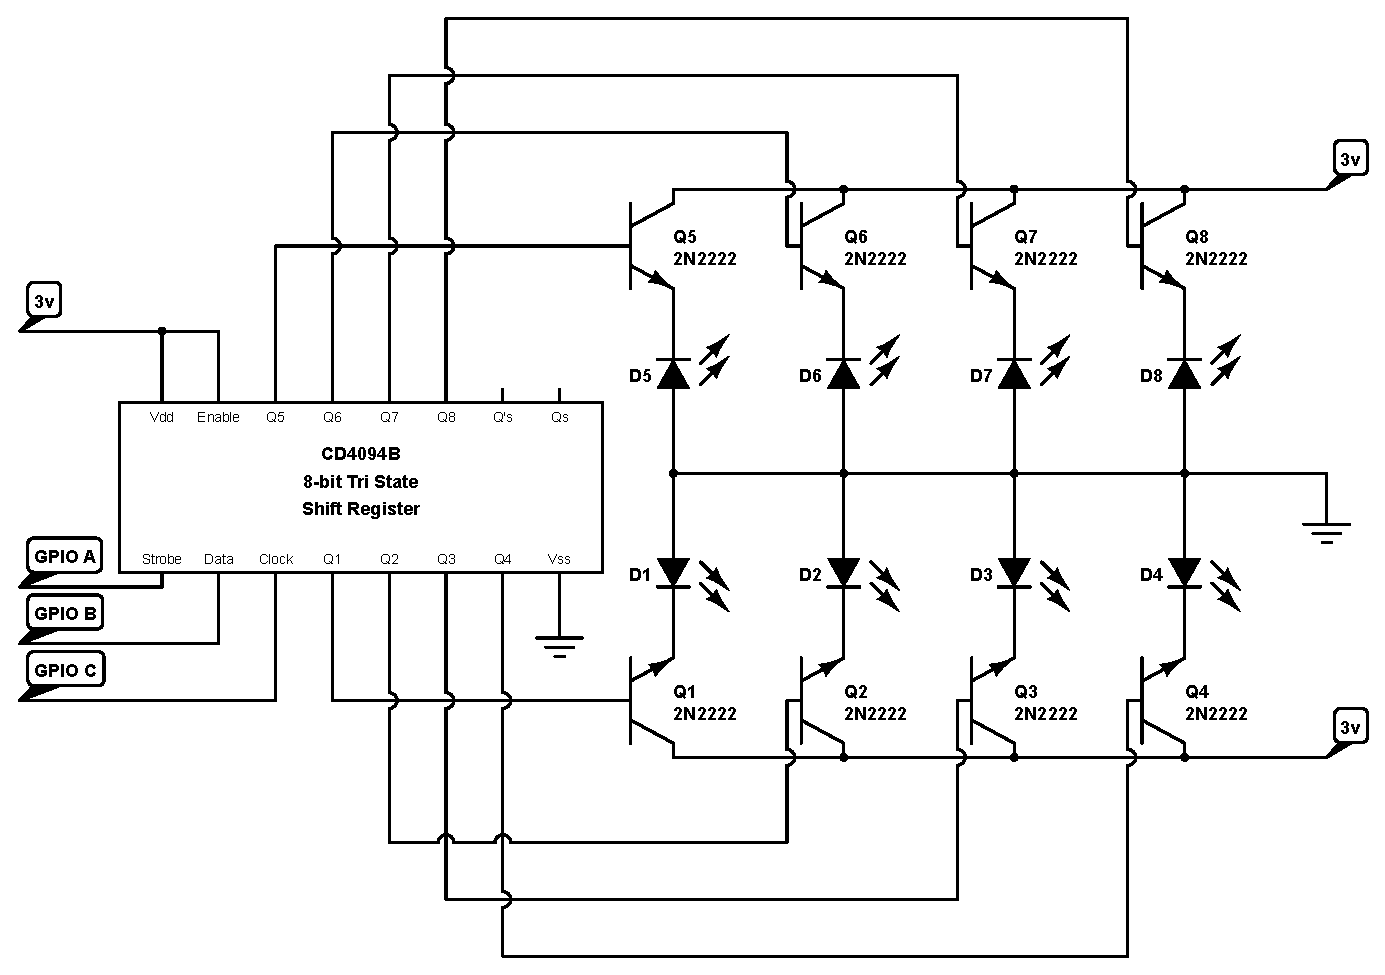
\includegraphics{assets/Shift-Register-Circuit.eps}
  \caption{Shift Register Circuit}
  \end{figure}
\item
  Implement the serial protocol needed to write to shift registers, and
  display some pattern that changes over time.
\item
  Detect the position of the button connected to GPIO C and use it to
  switch between two patterns.
\item
  Use fast switching to make the LEDs glow at different brightnesses
  while displaying some pattern, and having some interrupt based button
  interaction.
\item
  \textbf{Bonus:} Chain up two more shift registers, and use 8 RGB LEDs
  to display something.\footnote{The shift register data sheet has a
    diagram showing how to chain them for more storage.}
\end{enumerate}

\newpage

\section{Appendix}

\subsection{Development Environment Setup}

Executables destined for a microcontroller are somewhat different than
executables you intend to simply run. Where a normal executable will be
loaded by an OS, we need to make files that can be flashed, bit for bit,
onto the microcontroller's memory and run. To greatly simplify, an OS
takes an executable file, loads it into memory, looks for a pointer to
first instruction to execute in the executable's metadata, and starts a
process with the program counter set to that location. We have no OS to
offload a lot of this work to, we must build files that can be moved
directly onto the LPC's memory, with the starting instruction and other
features in the correct locations.

To do this we will be using a toolchain building applications for
\texttt{arm-none-eabi} , which means:

\begin{description}
\item[\texttt{arm}]
The CPU architecture we're building our applications for, this
determines the instructions and registers we have available, among other
things.
\item[\texttt{none}]
This is the operating system we're building for, in this case we're
building applications that run on the bare metal, with no intervening
OS.
\item[\texttt{eabi}]
The Embedded Application Binary Interface, this defines the conventions
for data types, file formats, stack usage, register usage, and function
parameter passing. Having a standard specification for this \footnote{The
  ARM EABI Standard :
  \url{http://infocenter.arm.com/help/topic/com.arm.doc.ihi0042e/IHI0042E_aapcs.pdf}}
means different libraries can be compatible with each other and your
code.
\end{description}

This toolchain comes with a number of tools, :

\begin{description}
\item[\texttt{as}]
The GNU assembler, which takes the assembly our compiler outputs, and
gives us ARM compatible machine code.
\item[\texttt{gcc}]
The GNU compiler collection which will take our C code, and turn it into
assembly.
\item[\texttt{gdb}]
The GNU debugger, you can use this to view your program as it's
executing, and see what its internal state is.
\item[\texttt{ld}]
The GNU linker, which takes compiled object code and can correlate all
the symbols and link it into a single executable.
\end{description}

There's also a number of less important tools from
\href{http://www.gnu.org/software/binutils/}{Gnu Binutils} that we'll be
using, all targeted to \texttt{arm-none-eabi}.

\subsubsection{Install Steps}

\paragraph{LPCXpresso}

In order to save building these tools ourselves, and to get the tools
which will allow us to flash the LPC through the proprietary LPC-Link
board, we'll have to download and install LPCXpresso, a set of tools and
Eclipse based IDE for working with the LPC.

To download the tools, visit the
\href{http://lpcxpresso.code-red-tech.com/LPCXpresso/}{LPCXpresso
Website} and register an account. Once you have confirmed your email,
you will be able to visit the
\href{http://lpcxpresso.code-red-tech.com/LPCXpresso/Downloads}{download
page}. There, download the latest version of LPCXpresso 5 for your
operating system and follow the provided installation instructions. Take
note of the installation directory, we'll use it later.

At this point, you can launch LPCXpresso and use it, if you would like.
It is recommended to launch it at least once and go through the software
activation step (no payment necessary, you are just verifying your email
again), as this upgrades the proprietary tools to handle a larger file
size.

\paragraph{Git}

You also need to install the \href{http://git-scm.com/downloads}{Git}
version control system.
\todo[size=\footnotesize]{Windows Instructions,and path changes.}

Git is a similar tool to SVN or CVS and allows you to store your code's
history and synchronize development with other programmers.

We use git to manage our build system.

\paragraph{CMake}

Next, install the \href{http://www.cmake.org/}{CMake} build system.
\todo[size=\footnotesize]{Windows Instructions,and path changes.}

CMake is a meta-build system. Instead of the standard UNIX
\texttt{make}, which directly compiles source code into the desired
output format, CMake instead generates one of many different types of
build systems,which are then used to perform the actual compilation.
This is useful for allowing different developers to use their preferred
development environment (POSIX, Visual Studio, Eclipse, etc\ldots{}). In
our example, we will use CMake to generate \texttt{Makefile}s.

\paragraph{MinGW}

If you're on windows, you should also install
\href{http://www.mingw.org}{MinGW}.

\todo[inline,size=\footnotesize]{Description, install steps}

\paragraph{UMD LPC Build}

The UMD LPC Build system was created in order to let us use the LPC with
our own choice of editors for coding, and a standard \texttt{gdb}
session to debug, instead of having to deal with a clumsy, hard to use
proprietary IDE.

To install, start by cloning the repository from github, while in
whatever directory you wish to work out of:

\begin{Shaded}
\begin{Highlighting}[]
    \KeywordTok{git} \NormalTok{clone https://github.com/rohit507/UMD-LPC1769-Build.git}
\end{Highlighting}
\end{Shaded}

This will have git retrieve the latest version of the build system from
github. We've also created a few submodules: separate repositories
storing single projects that let you manage them with git at the project
level instead of having to makes changes to the entire workspace
whenever you wish to change a project. To initialize these, run the
following:

\begin{Shaded}
\begin{Highlighting}[]
    \CommentTok{# Get submodules}
    \KeywordTok{cd} \NormalTok{GNU-LPC-Core/}
    \KeywordTok{git} \NormalTok{submodule init}
    \KeywordTok{git} \NormalTok{submodule update}
\end{Highlighting}
\end{Shaded}

Next we need to run the setup script and set a few internal variables so
CMake will know where it should look for the \texttt{arm-none-eabi}
toolchain, and proprietary tools. Here the \texttt{DLPCXPRESSO\_DIR}
variable should be set to the root directory under which all of the
necessary files can be found, this should contain the
\texttt{lpcxpresso}
binary.\todo[size=\footnotesize]{Add Windows to footnote} \footnote{On
  Linux or OSX it should look like
  \texttt{/usr/local/lpcxpresso\_5.1.2\_2065/lpcxpresso/}. On Windows it
  should look like \texttt{TODO: Insert actual path here}.}

\begin{Shaded}
\begin{Highlighting}[]
    \CommentTok{# Run setup script}
    \KeywordTok{cd} \NormalTok{_setup}
    \KeywordTok{cmake} \NormalTok{. -DLPCXPRESSO_DIR=}\KeywordTok{<}\NormalTok{LPCXpresso Root Dir}\KeywordTok{>}
\end{Highlighting}
\end{Shaded}

During setup, our script copied over the \texttt{CMSIS} library, this is
a library that provides some very basic LPC functionality, but we still
need to unzip it.

On Linux or OS X:

\begin{Shaded}
\begin{Highlighting}[]
    \CommentTok{# Extract CMSIS library .zip}
    \KeywordTok{cd} \NormalTok{..}
    \KeywordTok{unzip} \NormalTok{CMSISv2p00_LPC17xx.zip -d CMSISv2p00_LPC17x}
\end{Highlighting}
\end{Shaded}

On Windows:

\todo[inline,size=\footnotesize]{Add instructions here}

Now from within the \texttt{CMSIS} directory, we'll use CMake to
generate a build system.

On Linux or OS X:

\begin{Shaded}
\begin{Highlighting}[]
    \CommentTok{# Build CMSIS}
    \KeywordTok{cd} \NormalTok{CMSISv2p00_LPC17xx/}
    \KeywordTok{cmake} \NormalTok{. -G }\StringTok{"Unix Makefiles"}
    \KeywordTok{make}
\end{Highlighting}
\end{Shaded}

On Windows:

\todo[inline,size=\footnotesize]{Add instructions here}

Now we can build our skeleton project, which is the bare template all
your projects will be build from.

On Linux or OS X:

\begin{Shaded}
\begin{Highlighting}[]
    \CommentTok{# Build CMSIS}
    \KeywordTok{cd} \NormalTok{../Skeleton}
    \KeywordTok{cmake} \NormalTok{. -G }\StringTok{"Unix Makefiles"}
    \KeywordTok{make}
\end{Highlighting}
\end{Shaded}

On Windows:

\todo[inline,size=\footnotesize]{Add instructions here}

At this point all your installation steps are done and we can go over
basic usage, and workflow.

\subsubsection{Available Targets}

The default build target builds a .axf file with debug settings.

The following targets are provided:

\begin{description}
\item[\texttt{lst}]
Generate a .lst file, which includes an overview of all the sections and
symbols in your output, along with a complete disassembly.
\item[\texttt{hex} and \texttt{bin}]
Generate alternate formats of the normal .axf output, which may be
useful if you want to use other tools.
\item[\texttt{boot}]
Boot the LPC-Link board. This is required before flashing or debugging
the microcontroller using the LPC-Link board.
\item[\texttt{flash}]
Write the currently built output to the microcontroller. The
microcontroller immediately starts running after the flash is complete.
\item[\texttt{flash-halt}]
The same as \texttt{flash}, but the microcontroller is left in a stopped
state.
\item[\texttt{gdb}]
Launch a gdb session. Complete debug information is also setup. Note
that it is not always simple to restart the current program.
\texttt{run} (\texttt{r}) will work for some programs, and sometimes,
using \texttt{jump} (\texttt{j}) to jump to the entry point of the
current image (found with \texttt{info files}) works. However, none of
these completely reset the chip - the only command that will is the
\texttt{load} command, however that will flash the entire image to the
chip again, which may take a while for projects with large compiled
binaries. Also note that some circuits (particularly when interfacing
with other chips that have their own state) may require completely
unplugging the circuit between program runs.
\end{description}

If using makefiles, these are directly accessible as \texttt{make lst},
etc. (run in the root directory of the desired project). If you are
using a build system based around IDE project files (such as Eclipse or
Visual Studio), the targets should be accessible from a menu.

\subsubsection{Typical Workflows}

These sections detail how to do many common tasks. They are written
under the assumption that a Makefile build system is being used, but the
calls to \texttt{make} can all be substituted with the appropriate
action in any other chosen build system.

\paragraph{Start a new project (by forking):}

First go \href{https://github.com/rohit507/GNU-LPC-Skeleton}{here} and
fork a new project.

In your terminal:

\begin{Shaded}
\begin{Highlighting}[]
    \KeywordTok{git} \NormalTok{submodule add http://github.com/yourname/newprojectname}
    \KeywordTok{git} \NormalTok{add .gitmodules}
    \KeywordTok{git} \NormalTok{commit -m }\StringTok{"Added a submodule for NewProjectName"}
    \KeywordTok{git} \NormalTok{submodule update}
    \KeywordTok{cd} \NormalTok{NewProjectName}
    \KeywordTok{YOUR_EDITOR} \NormalTok{CMakeLists.txt}
    \CommentTok{# Edit CMakeLists.txt, and change the project name.}
    \KeywordTok{cmake} \NormalTok{. -G }\StringTok{"Unix Makfiles"}
    \KeywordTok{make}
\end{Highlighting}
\end{Shaded}

\paragraph{Start a new project (by copying):}

In your terminal:

\begin{Shaded}
\begin{Highlighting}[]
    \KeywordTok{cp} \NormalTok{-R Skeleton/ NewProjectName}
    \KeywordTok{cd} \NormalTok{NewProjectName}
    \KeywordTok{YOUR_EDITOR} \NormalTok{CMakeLists.txt}
    \CommentTok{# Edit CMakeLists.txt, and change the project name.}
    \KeywordTok{cmake} \NormalTok{. -G }\StringTok{"Unix Makfiles"}
    \KeywordTok{make}
\end{Highlighting}
\end{Shaded}

\paragraph{Work on an existing project}

In your terminal:

\begin{Shaded}
\begin{Highlighting}[]
    \CommentTok{# Open source files in editor and make + save changes}
    \KeywordTok{make}
\end{Highlighting}
\end{Shaded}

\paragraph{Enabling semihosting for a project}

Open a project's \texttt{CMakeLists.txt} file and uncomment the
following line:

\begin{Shaded}
\begin{Highlighting}[]
    \KeywordTok{set}\NormalTok{(SEMIHOSTING_ENABLED True)}
\end{Highlighting}
\end{Shaded}

Then just rebuild the project, and semihosting messages will be viewable
in gdb.

\paragraph{Adding compiler options}

All compiler options are configured in
\texttt{Platform/LPC1769\_project\_default.cmake}. To add compiler
options to a single project, you can use CMake's
\texttt{add\_definitions} command in that project's CMakeLists.txt.

In your \texttt{CMakeLists.txt}:

\begin{Shaded}
\begin{Highlighting}[]
    \KeywordTok{add_definitions}\NormalTok{(}
      \NormalTok{-Wall}
      \NormalTok{-Werror}
      \NormalTok{-02}
      \CommentTok{# Add more compiler flags here}
    \NormalTok{)}
\end{Highlighting}
\end{Shaded}

\paragraph{Add a source file to a project}

When adding source files to a project, remember to open that projects
CMakeLists.txt and add the file to the \texttt{SOURCES} variable.

In your \texttt{CMakeLists.txt}:

\begin{Shaded}
\begin{Highlighting}[]
    \KeywordTok{set}\NormalTok{(}\OtherTok{SOURCES}
      \NormalTok{src/cr_startup_lpc176x.c}
      \NormalTok{src/project.c}
      \CommentTok{# Add more source files here}
    \NormalTok{)}
\end{Highlighting}
\end{Shaded}

\paragraph{Flash a program}

In your terminal:

\begin{Shaded}
\begin{Highlighting}[]
    \CommentTok{# Plug in the LPC1769}
    \KeywordTok{make}
    \KeywordTok{make} \NormalTok{boot}
    \KeywordTok{make} \NormalTok{flash}
\end{Highlighting}
\end{Shaded}

\paragraph{Debug a program}

In your terminal :

\begin{Shaded}
\begin{Highlighting}[]
    \CommentTok{# Plug in the LPC1769}
    \KeywordTok{make}
    \KeywordTok{make} \NormalTok{boot}
    \KeywordTok{make} \NormalTok{gdb}
\end{Highlighting}
\end{Shaded}

In GDB:

\begin{Shaded}
\begin{Highlighting}[]
    \NormalTok{b main}
    \NormalTok{load}
    \NormalTok{c}

    \CommentTok{# Make changes to the program}

    \NormalTok{make}
    \NormalTok{load}
    \NormalTok{c}
\end{Highlighting}
\end{Shaded}

For more information on how use GDB refer to a
\href{http://www.cs.cmu.edu/~gilpin/tutorial/}{simple tutorial} or the
\href{https://sourceware.org/gdb/current/onlinedocs/gdb/}{full user
manual}.

\newpage

\todototoc
\listoftodos

\end{document}
